\documentclass[11pt]{article}
\usepackage{libertine}
\usepackage{paralist}
\usepackage{graphicx}
\usepackage{algorithm,algpseudocode}
\usepackage{tikz}
\usepackage{xcolor,colortbl}
\usepackage{wrapfig}
\usepackage{url}
\usepackage{hyperref}
\usepackage{amsmath,amssymb,amsthm}
\usepackage{xspace}

\usepackage{cleveref}

\DeclareMathOperator*{\argmin}{argmin}


\topmargin 0pt
\advance \topmargin by -\headheight
\advance \topmargin by -\headsep

\textheight 8.9in

\oddsidemargin 0pt
\evensidemargin \oddsidemargin
\marginparwidth 0.5in

\textwidth 6.5in


\pagestyle{empty}
\setlength{\oddsidemargin}{0in}
\setlength{\topmargin}{-0.8in}
\setlength{\textwidth}{6.8in}
\setlength{\textheight}{9.5in}


\newtheorem*{definition*}{Definition}

\newcommand{\psnumber}{3}
\newcommand{\duedate}{Tuesday, 4 March 2025}

\begin{document}


\setlength{\parindent}{0in}
\addtolength{\parskip}{0.1cm}
\setlength{\fboxrule}{.5mm}\setlength{\fboxsep}{1.2mm}
\newlength{\boxlength}\setlength{\boxlength}{\textwidth}
\addtolength{\boxlength}{-4mm}
\begin{center}\framebox{\parbox{\boxlength}{\bf
Introduction to Algorithms \hfill Homework~\#\psnumber\\
CS 4820, Spring 2025 \hfill Due:~\duedate}}\end{center}
\vspace{5mm}

\theoremstyle{plain}
\newtheorem{theorem}{Theorem}[section]
\newtheorem{lemma}[theorem]{Lemma}
\newtheorem{corollary}[theorem]{Corollary}
\newtheorem*{theorem*}{Theorem}
\newtheorem*{lemma*}{Lemma}




\def\ind{\hspace*{0.3in}}
\def\gap{0.1in}
\def\bigap{0.2in}
\newcommand{\Xomit}[1]{}
\newcommand{\hwprob}[2]{{\bf (#1)} {\em (#2)}~~~~~}

{\bf Instructions:}
\begin{compactitem}
    \item Solve the following problems to the best of your ability.  The problems are challenging, by design---it's ok if you cannot solve them all.  If you are stuck, {\bf stop by Office Hours} for help getting unstuck.
    \item Submit your completed solutions on {\bf Gradescope}.  Solutions should be typeset (using LaTeX) as a single pdf file. For each problem, mark the start and end of your solution within the file.
    \item Collaboration is encouraged while solving the problems!  You may discuss the problems with anyone in the class, but significant collaborations (at the level of drawing diagrams or writing out ideas) should be limited to groups of at most 3 students. Additionally, you must:
    \begin{compactenum}
        \item list the names of all (up to 2) significant collaborators;
        \item write up your solutions, independently from collaborators, in your own words.
    \end{compactenum}
    Do {\bf not} solicit help from people outside of the class 
    (i.e., beyond classmates and course staff).
    \item If a problem asks you to {\bf design and analyze} an algorithm, you must:
    \begin{compactenum}
        \item Clearly describe your algorithm (in English and/or pseudocode).
        \item Prove the algorithm's {\bf correctness}.
        \item Analyze the algorithm's asymptotic {\bf running time}.
    \end{compactenum}
    \item In your solutions, you may appeal to any algorithm from this semester's CS 4820 lectures, textbook, and assigned readings, without re-proving correctness and running time.  If you use a lemma from 4820 materials or a prerequisite class (CS 1110, 2110, 2800, 3110) without proof, you must {\bf cite your source}.
\end{compactitem}

\vskip \gap
\hrulefill
\vskip \gap


\hwprob{1}{8 points}
\textbf{Campsite Assignments.}

Treman State Park is unveiling a new set of scenic campsites. 
Given the popular demand, you’ve been hired to manage the campsite assignment system.
Each weekend, there are $n$ camping groups who want to visit every one of $n$ scenic sites, split across Saturday and Sunday.
Every group $g$ submits an itinerary consisting of the following information:
\begin{compactitem}
\item a starting time $s_g$ on Saturday, when the group $g$ will leave from the parking lot, denoted as $c_0$;
\item an ordered list $L_g$ of all the scenic sites, where $L_g[i] = c_j$ indicates that the site $c_j$ will be the $i$th site visited by group $g$;
\item an ordered list of times $T_g$, where $T_g[i]$ indicates the time that group $g$ will take to travel from site $L_g[i-1]$ to $L_g[i]$.\footnote{You should assume that every itinerary is short enough that, in principle, it could be completed in a single day. Nevertheless, every group wants to camp overnight at one of the campsites.}
\end{compactitem}

Your job is to assign groups to camping sites respecting a few key constraints:
\begin{compactitem}
    \item Exactly one group is assigned to each site.
    \item Once a group arrives at their assigned campsite, they stop for the night, resuming the itinerary in the morning.
    \item To respect each group’s privacy, once a group has stopped at their assigned campsite $c$ for the night, no other group should pass through site $c$, until the following day.\footnote{It is not a privacy violation, however, if two groups arrive at a campsite at the same time, and one stays to camp while the other continues hiking.}
\end{compactitem}

\textbf{Design and Analyze} a polynomial-time \textbf{reduction} from the problem of campsite assignments to the \textsc{StableMatching} problem.

\newpage
% Solution for Problem 1.
{\color{blue}
\emph{Solution.}

\textbf{Algorithm.}

We reduce to the \textsc{Stable-Matching-Problem} by constructing preferences for the groups and sites:
\begin{itemize}
  \item group $g$ prefers campsites in ascending order according to $L_g$ (i.e. earliest site is most preferred);
  \item site $S$ prefers a group $g$ to a group $h$ if group $g$ plans to arrive at $S$ \emph{later} than group $h$.
\end{itemize}

If there are any ties in the preference list for sites, we will just break them arbitrarily. We then return the assignment of groups to sites obtained by running Gale-Shapley on these preference lists with groups being proposers \& sites being receivers (or vice versa).

\textbf{Correctness.}
% \emph{A quick aside on reductions.} Suppose we have a reduction from \textsc{Problem-A}  to \textsc{Problem-B}. Specifying a reduction requires us to specify an algorithm $\textsc{Alg}$ for solving \textsc{Problem-B} and specifying two transformations: a function $f$ that transforms an instance $I$ of \textsc{Problem-A} to an instance $I'$ of \textsc{Problem-B} and a function $g$ that transforms a solution to instance $I' = f(I)$ of \textsc{Problem-B} to a solution of instance $I$ of \textsc{Problem-A}. This is the sense in which we are seeking a `one-to-one' correspondence (note how this is weaker than asserting that $f,g$ are inverses of one another or that these transformations are injective/surjective). In principle, proving correctness necessitates showing the following equivalence holds: for any instance $I$ of \textsc{Problem-A} there exists a solution $X$ for $I$ if and only if $I' = f(I)$ is an instance of \textsc{Problem-B} having a solution $\textsc{Alg}(I')$ such that $g(\textsc{Alg}(I'))$ is a solution for the original instance $I$.
%
% - if there is a solution to the original you can find a solution to the converted instance (completeness) (Yes instance => Yes instance) (If privacy exists then gale shapley returns a stable matching) (if tiling exists then max-bipartite matching)
%
% - when you find a solution to reduced problem you solve original 

First, note that Gale-Shapley, given strict preference lists, always returns a stable matching. So, our algorithm always terminates. Next, we wish to show that the assignment of groups to sites is privacy-preserving.

\setcounter{section}{1}
\begin{lemma}
  The stable matching returned by the algorithm respects privacy constraints.
\end{lemma}
\begin{proof}
  Suppose for contradiction that the assignment returned violates the privacy constraint. That is the matching contains the pairs $(g, s)$ and $(g', s')$ however group $g$, before it reaches $s$, travels through $s'$ after $g'$ has arrived. In terms of the preferences we construct, this implies that $g \succ_{s'} g'$ and $s' \succ_{g} s$ which implies that $(g, s')$ is an instability. This is a contradiction! 
\end{proof}

\textbf{Runtime.}

Each group's preferences are already specified by the provided itenary. 

We have to do more work to construct the preference list for each site. We start by computing for every group $g$, its arrival time at $a_i^G$ for each site $L_g[i]$. This can be done by making a linear pass over $T_g$ to computing $a_i^G = s_g + \sum_{j \le i} T_g[i]$. Then for every group $g$, add $(g, a_i^G)$ to a list associated with site $L_g[i]$. Finally, we sort the list for each site based on descending arrival times. 

The linear pass takes $\mathcal{O}(n)$ and we sort $n$ different lists, which takes $\mathcal{O}(n^2 \log n)$ overall. Running Gale-Shapley itself takes $\mathcal{O}(n^2)$. So, the overall running time is $\mathcal{O}(n^2 \log n)$.
}

\clearpage















\hwprob{2}{10 points}
\textbf{Implementing the Reduction.}

In this problem, you are asked to code up portions of the Gale-Shapley algorithm for the \textsc{StableMatching} problem, and your reduction from \textbf{(1)}.
To help with the task, we provide starter code in a file called \texttt{main.py}.
The starter code provides the implementation of key classes that will be helpful for implementing Gale-Shapley algorithm.
There are two comment blocks that include the phrase, \texttt{\#YOUR CODE HERE\#},
where you should add your implementation of:
\begin{compactitem}
    \item The core logic of the Gale-Shapley algorithm; and
    \item Your reduction from \textbf{(1)}.
\end{compactitem}
In all, you will complete a program that solves the campsite assignment problem.

You are responsible for testing your code for correctness!
We provide a few public test cases, which are primarily meant to check for correct input-output formatting.
Please be aware that these tests are \textbf{not} exhaustive. Your code will be subjected to more rigorous private test cases during grading.



\paragraph{Input Format.}
The input to campsite assignment problem is given in the following format:
\begin{compactitem}
    \item The first line is an integer \textit{n}, the number of groups/campsites;
    \item Then, of the next $n$ lines, the $g$th line specifies the ordered list of campsites $L_g$ for group $g = 1,\hdots,n$;
    \item Then, of the next $n$ lines, the $g$th line specifies the start time $s_g$ followed by the travel times $T_g$ for group $g = 1,\hdots,n$.
\end{compactitem}
The starter code provides a function for reading the input into useful data structures.




\vskip\gap
\textbf{Example input.}
Consider the following instance with $2$ groups $\{A,B\}$ and sites $\{c,d\}$.
To specify the instance, we give the location lists, the start times, and travel time lists for each group.
\begin{align*}
    \text{Group } A:& &L_{A} = \langle c,\,d \rangle& &s_{A} = 8 \quad \text{and} \quad &T_{A} = \langle 1,\,2 \rangle\\
    \text{Group } B:& &L_{B} = \langle c,\,d \rangle& &s_{B} = 9 \quad \text{and} \quad &T_{B} = \langle 2,\,3 \rangle
\end{align*}


Given these groups, sites, and lists, the input would be specified as follows.
\begin{verbatim}
2
1 2
1 2
8 1 2
9 2 3
\end{verbatim}
The first line tells us there are $n = 2$ camping groups ($A$ and $B$) and $2$ campsites ($c$ and $d$). The next two lines describe $L_A$ and $L_B$ (where $c$ and $d$ are encoded numerically as \texttt{1} and \texttt{2}).
The final two lines encode $s_A$ followed by $T_A$ and $s_B$ followed by $T_B$.


\paragraph{Output Format.}
Given $n$ groups and campsites, the output format consists of $n$ lines, where the $g$th line begins with the number \texttt{g} followed by the number of the campsite that group $g$ is assigned.
The starter code provides a function that handles writing the assignment to \texttt{stdout}.
Be careful to avoid extra spaces or any other extraneous output!












\paragraph{Submission.}
Submit your assignment on Gradescope as a single file called \texttt{main.py}.

\clearpage
\hwprob{3}{12 points} \textbf{Domino Tilings.}

In Lecture 1, we saw the definition of a tiling:
a \emph{tiling} of a shape $S$ with a tile $t$ is an arrangement of non-overlapping copies of $t$ that exactly cover the area of $S$.
In particular, we considered the \textsc{DominoTiling} Problem, where
dominoes are tiles of dimension $2 \times 1$ (or rotated, $1 \times 2$).

We say a shape $S$ is a \emph{sub-grid} if its area can be broken down into contiguous $1\times 1$ squares, which are aligned on an integer grid.
In particular, the shape $S$ can be described by a collection of integer coordinates $(x,y) \in \mathbb{Z}^2$, indicating the lower left corner of a unit square contained by $S$.





\vskip\gap

The \textsc{DominoTiling} Problem asks:
\begin{quotation}
\emph{Given a sub-grid shape $S$, does there exist a tiling of $S$ using dominos?}
\end{quotation}

\begin{figure}[h!]
    \centering
    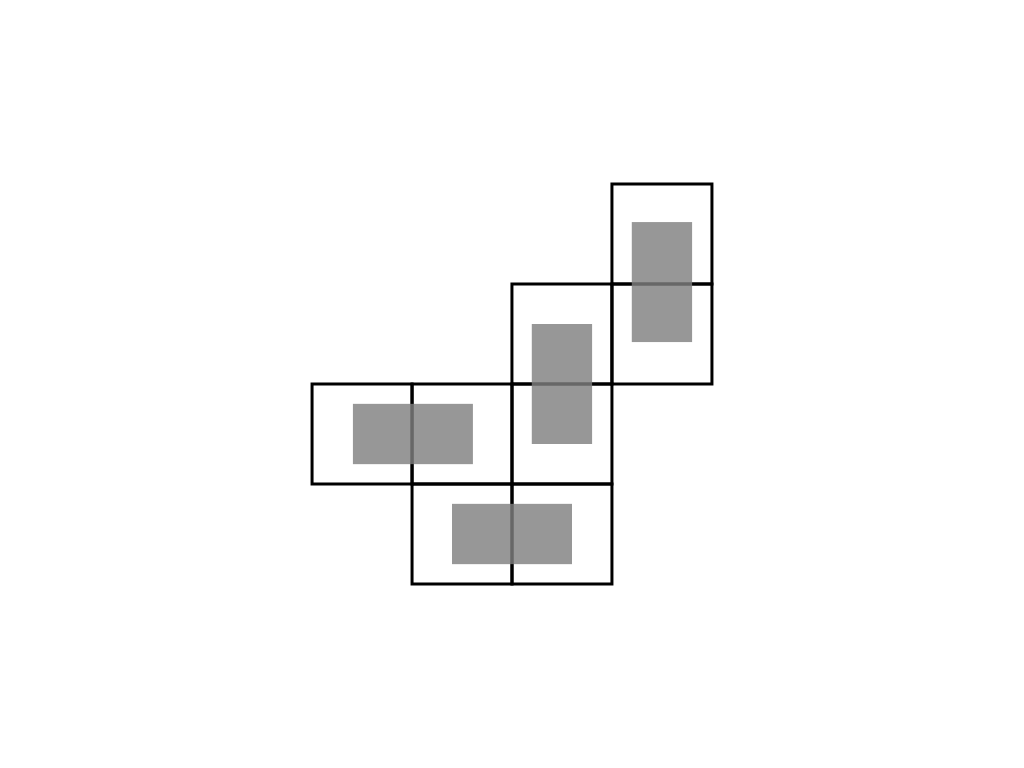
\includegraphics[width=0.3\linewidth]{tiled-YES.png}
    
\includegraphics[width=0.3\linewidth]{shape-NO.png}
    
\includegraphics[width=0.3\linewidth]{Big-NO.png}
    \caption{Example \textsc{DominoTiling} instances.
    The shape on the far left CAN be tiled with dominos, whereas the shapes in the center and on the far right CANNOT be tiled with dominos.}
    \label{fig:shapes}
\end{figure}

\textbf{Design and Analyze} a polynomial-time algorithm to solve the \textsc{DominoTiling} Problem.

Assume that the input is a sub-grid shape specified by a set of coordinates.
$$S = \{ (x,y) : \textrm{ $1 \times 1$ square area starting at $(x,y)$ is included in the shape } \}$$
Concretely, the center example from Figure~\ref{fig:shapes} could be specified as follows.
$$S = \{(0,0), (1,0), (2,0), (1,1), (2,1), (2,2), (3,2), (3,3)\}$$
Your algorithm should run in polynomial time in the area of the shape $S$.

% Solution for Problem 3
{\color{blue}
\emph{Solution.}

\textbf{Algorithm.} 

We start by constructing a graph $G$ with vertex set $V = S$ and edgeset 
\begin{align*}
 E = \{ (x, y) \subseteq S^2 \, \mid \, |x_1 - y_1| + |x_2 - y_2| = 1 \}.
\end{align*}
Intuitively, $G$ is just a convenient representation of our board as a ``grid graph''. Each vertex is a tile and the condition that edges only exist between tiles whose coordinates differ by exactly $1$ in one of the directions corresponds to tiles that are adjacent to one another. It is also useful to think of these edges as being \emph{potential} dominoes we may place.

We then partition $V = W \sqcup B$ via the following rule 
\begin{align*}
  (x_1, x_2) \in W \text{ iff } x_1 + x_2 = 0 \mod 2.
\end{align*}

Finally, we compute $M = \textsc{Max-Bipartite-Matching}(G)$. If $|M| \ge |S|/2$ then our algorithm claims that a tiling exists, otherwise we say that no valid tiling exists. 

\textbf{Correctness.}

First, we should verify that $G$ is bipartite so that the reduction to $\textsc{Max-Bipartite-Matching}$ even makes sense. 

\setcounter{section}{3}
\begin{lemma}
$G$ is bipartite.
\end{lemma}
\begin{proof}
  Suppose that $(x, y) \in E$ then we have, by construction of our edge set,
\begin{align*}
  (x_1 + x_2) - (y_1 + y_2) = \pm 1 = 1 \mod 2. 
\end{align*}

So, $x$ and $y$ cannot be in the same set of our partition $V = W \sqcup B$. \\
\end{proof}

Note now that the condition that $|M| \ge |S|/2$ is equivalent to saying that $M$ is a perfect matching. This follows from noting that $2 |M|$ is the number of vertices that are adjacent to an edge in the matching $M$ and $|S|$ is the total number of vertices in $G$.

We now finish proving correctness of the reduction by showing a one-to-one correspondence between the instances of our two problems.

\begin{lemma}
  If there exists a perfect matching $M$ on the graph $G$ then there is a valid tiling of the $S$ by dominoes. 
\end{lemma}
\begin{proof}
  Given the perfect matching $M$, each edge $e \in M$ identifies a donimo-- particularly, by identifying the two tiles covered by the domino. Since edges only exist between adjacent tiles, we only identify valid dominoes. Furthermore, note that as $M$ is a perfect matching, every vertex in $V = S$ is adjacent to exactly one edge in $E$. In terms of our dominoes, this implies that every tile is covered by exactly one domino. That is, the entire shape is tiled with dominos and no two dominos overlap. \\
\end{proof}

\begin{lemma}
  If there exists a valid tiling of $S$ by dominoes then there exists a perfect matching $M$ on the graph $G$. 
\end{lemma}
\begin{proof}
  Let $T$ be such a tiling of dominos that exactly covers $S$. Define $M \subseteq E$ as follows:
  \begin{align*}
    M = \{ (x, y) \in E \, \mid \, \text{ there is a domino in } T \text{ covering the tiles } x, y \}.
  \end{align*}

  This is well defined as dominoes can only cover adjacent tiles and edges in $G$ only exist between adjacent tiles. Furthermore, note that as no two dominoes cover the same trial, no two edges in $M$ are adjacent to the same vertex. By definition, this makes $M$ a matching. As every tile $x \in S$ in our shape is covered by some domino in $T$ covering $x$ and some other tile $y$, we note that every vertex in $V$ is adjacent to an edge $(x, y) \in M$. Thus, $M$ is a perfect matching. \\
\end{proof}

\textbf{Runtime.}

Let $n = |V| = |S|$.

Constructing the graph $G$ take $\mathcal{O}(n)$: The vertex set $V$ is just $S$. Computing the edgeset also takes $\mathcal{O}(n)$ as we may just iterate over every vertex and create (at most) $4$ edges for it.

The runtime of $\textsc{Max-Bipartite-Matching}(G)$ is $\mathcal{O}(n^2)$. 

Thus, the overall runtime of our reduction is $\mathcal{O}(n^2)$.
}




\end{document}

